\chapter{EVENT LOCALIZATION}
This section of thesis considers the problem of localization: the objective is to detect where an action of interest occurs. The expected output of such a system is typically a subvolume encompassing the action of interest. Since a localized action only covers a fraction of the spatio-temporal volume in a video, the task is considerably more challenging than event classification. Some of the common startergies that are tried on this kind of problems are efficient sub-window search ~\citep{subwindowsearch},"selective search" stratergy ~\citep{selectivesearch}  and a recent by ~\cite{tubelet}, but these either does a exhaustive search or does a iterative merging of the supervoxels. 

\section{Background Subtraction Techniques} 
\par Event localization can be performed by determining the position with pixel changes and understanding the motion relativity ~\citep{Basharat08}, where all components corresponding to an event show a similar flow of pixels. Following approach works significantly well in surveillance data but fails terribly in case human event detection. Later realized that, by eliminating the background(static parts) of the visual frame,  possible event locations can be retained.  Several background subtraction technique are eminent in the \cite{Piccardi04}, among these some apply on static image while others on dynamic video. In case of our application we can blend both these approaches to generate more reliable event detectors.

\subsection{Frame Differencing (FD)}
A very common approach for performing the moving object segmentation is using frame differencing but these approach is very sensitive to small changes and yields lots of noise when a camera is in motion. A simplest way to implement this technique is by computing the absolute difference of gray scale/intesity values two consecutive frames. Consider $P(p_x,p_y,t)$, intesity of pixel $(p_x,p_y)$ at frame t, then pixel $(p_x,p_y)$ that is considered foreground when absolute difference is above a threshold,$$\vert P(p_x,p_y,t+1) - P(p_x,p_y,t)t\vert > T$$.
\par The robustness of this method depends on speed of forground elements. Faster movements may require higher thresholds to reduce the noise.  An alternate approach is to replace difference of a single previous frame  by an average of multiple previous frames, still results are noisy and not reliable.

\subsection{Mixture of Gaussian (MOG)}
This is one of the well known method of extracting foreground information. \cite{kaew} model each background pixel by a mixture of N Gaussian distributions. The weights of the mixture represent the time proportions that those colors stay in the scene. The probable background colors are the ones which stay longer and more static. At any instance $i$ a particular pixel $(p_x,p_y)$ has color space represented as $V(p_{x},p_{y},i)$, history of the pixels are given by 
$$X_{1},..,X_{t} = {V(p_{x},p_{y},i)~:~1\le i \le t }$$
The history is modeled by mixture of N gaussian mixtures,
$$P(X_{t})=\Sigma_{i}^{N}w_{(i,t)}\eta(X_{t},\mu_{(i,t)},\Sigma_{(i,t)})$$
\par $w_{(i,t)}$,$\mu_{(i,t)}$,$\Sigma_{(i,t)}$ are weight,mean and covariance of the $i^{th}$ Gaussian in the mixture at time $t$ respectively and where $\eta$ is gaussian density function. General principle behind this approach is that when a new object occludes the background object, it will not match one of the existing distributions. Instead will result in either the creation of a new distribution or the increase in the variance of an existing distribution. The variance of the moving object is expected to remain larger than a background pixel until the moving object stops.


\subsection{Eigen subtraction (ES)}
An alternate approach named eigen background subtraction was seen to be more elegant. A sample of N images of the videos are obtained, mean background image $\nu_b$ is computed and all images are mean normalized  $X$. Principal component analysis on the mean normalized images is performed , idea is, that a high-dimensional images are often described by correlated variables and only a few meaningful dimensions account for most of the information. But performing PCA is not straightforward, consider 100 images of dimension 100x100 pixels, then the dimension of generated covariance matrix would be 10000x10000, i.e roughly 0.8 GB (considering 64 bit float values). Solving this is not feasible, hence a trick from linear algebra that for a MXN matrix with $M>N$, can at most have N-1 non-zero eigen values ~\cite{Duda01} can be used. Eigen decomposition of $X^TX$ is carried out:
$$X^TX\nu_i=\lambda_i\nu_i$$
$$XX^T(X\nu_i)=\lambda_i(X\nu_i)$$
The orthonormal eigen vector of $XX^T$ is found out by normalizing $X\nu_i$ to unit length. Once eigen vectors of $XX^T$  are computed, projection of the current frame $F$ on the eigen vector with top eigen values are determined, and the reconstructed frame $F'$ is obtained by using the projection coefficients and the eigen vectors. The difference $F-F'$ would correspond to the mask on the moving object. 

\begin{figure}[htpb]
   \begin{center}
	    \includegraphics[width=0.75\textwidth]{snaps/bgsub/results.eps}     
     \caption {Background subtraction techniques on multiple video classes}
   \label{fig:bgsub}
   \end{center}
 \end{figure}
\par Results of foreground mask obtained using FD, ES and MOG are shown in Figure \ref{fig:bgsub}. Eventhough MOG is most preferred, but found it provide sparse and not a clear boundary in most of the sample videos. In the example of "dance", the FD yields extraneous pixels due to camera movemnet in between two dancers, which are not evident in ES and MOG. While it produces spurious pixels for the "pommello" video, because of sharp background. All methods terribly fail incase of grainy videos, hence background subtraction alone cant be suffice for the event localization.

\section{Saliecny Detection}
Visual saliency is the distinct subjective perceptual quality which makes some items in the world stand out from their neighbors and immediately grab our attention.
As we had discussed earlier about the different techniques to extract the eminent pixels which are in motion, sometimes pixels which are stationary and quite distinct might also play a important role in the the activity recognition. These approaches are considered during the process attention modelling. Most of saliency estimations techniques in literature have the following five steps,

\subsubsection{Step 1: Color equalization:} This is performed by removing the tail in the color histogram. It helps improving the contrast in the image. In the implmentation color equalization is done on each channel separetely so that all channels can be provided to the segmentation algorithm.

\subsubsection{Step 2: SLIC-based segmentation:}  It is a simple linear iterative clustering that clusters pixels in the combined five-dimensional color and image plane space to efficiently generate compact, nearly uniform superpixels. Any slic based clustering algorithm takes two parameters number of super-pixels and compactness of each superpixel. According to \cite{slic}, slic is fastest and most memory efficient compared to  other segmentation technique like graph-cut, quick shift segmentation technques. Segmentation reduces the number of computation in the subsequent stages.

\subsubsection{Step 3: Extract segment properties:} Extracting features of the region that are used in computing the saliecny of each regions. Some features that are considered in the implementation are color based features (LAB,RGB) and texture based features (GLCM,Texture Flow).

\subsubsection{Step 4: Compute~saliency:} Saliecny estimation techniques can be broadly categorized into bottom-up, top-down and information maximization based on algorithmic computation. Earliest saliency based attention modelling was proposed by \cite{itti}. It was inspired by the behavior and the neuronal architecture of the early primate visual system.

\subsubsection{Step 5: Saliency cut:} Saliency maps are generally thresholded to obtain the salient mask. In the implementation, grab-cut\citep{grabcut} performs segmentation by modeling foreground and background based on saliency estimation to obtain the mask where higher saliency  contemplate foreground while lower saliency estimate corespond to background. Once saliency mask are obtained few morphological operation are applied to remove the salt and pepper noise.

\begin{figure}[htpb]
   \begin{center}
	    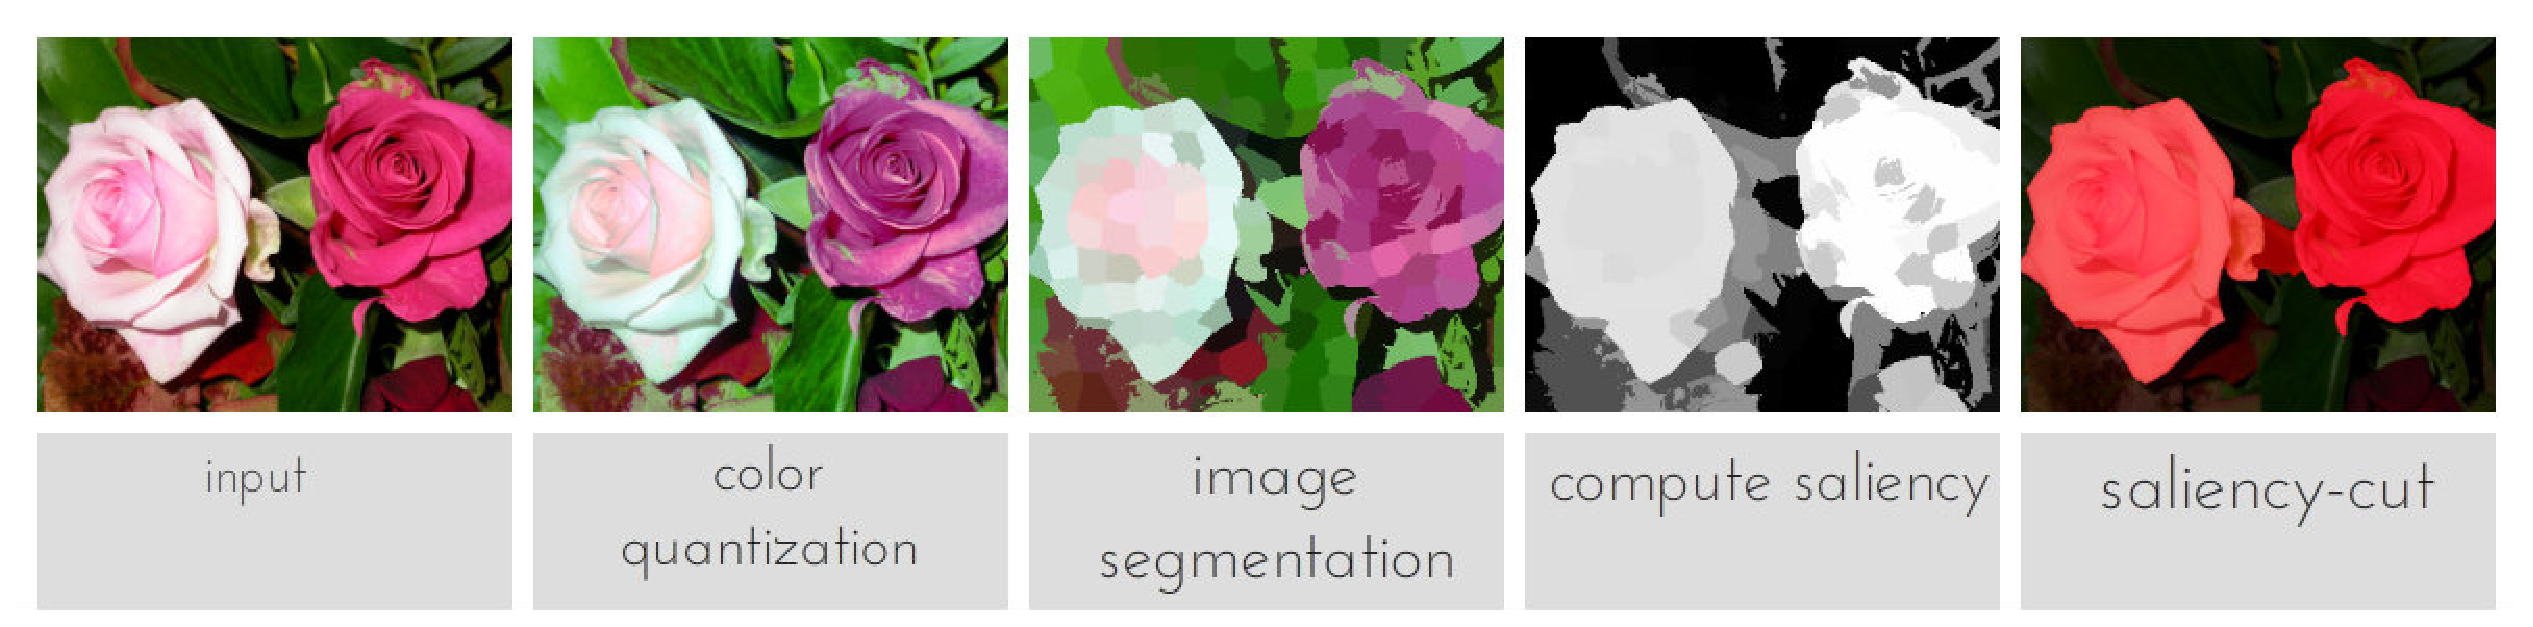
\includegraphics[width=0.95\textwidth]{snaps/sal/saliency.eps}     
     \caption {A general approach for saliency estimation}
   \label{fig:bgsub}
   \end{center}
 \end{figure}

\par Some of the saliency estimation techniques that were studied in the thesis are,
\subsection{Hierarchical Color Based}
It is a top-down approach for computing saliency. In this approach we hierarchically set saliency map of improbable salient pixels to zero at every iteration.

\subsection{Contxt Aware Based}
\subsection{Spectral Distribution Based}
\subsection{Regional Contrast}



